\documentclass{article}

\usepackage{amsmath}
\usepackage{color}
\usepackage[hidelinks]{hyperref}
\usepackage{listings}
\usepackage{tikz}
\usepackage{tikz-qtree}
\usepackage{verbatim}

% Colors copied from https://stackoverflow.com/questions/3175105/
\definecolor{dkgreen}{rgb}{0,0.6,0}
\definecolor{gray}{rgb}{0.5,0.5,0.5}
\definecolor{mauve}{rgb}{0.58,0,0.82}

\lstset{
	aboveskip=5mm,
	belowskip=5mm,
	basicstyle={\large\ttfamily},
	columns=flexible,
	language=Lisp,
	numbers=left,
	showstringspaces=false,
	% Style copied from https://stackoverflow.com/questions/3175105/
	numberstyle=\normalsize\color{gray},
	keywordstyle=\color{blue},
	commentstyle=\color{dkgreen},
	stringstyle=\color{mauve},
}

\bibliographystyle{acm}

\title{The Ergonomics of Faceted Execution}
\author{Ian Fisher \\ \\ Advised by Kristopher Micinski \\ \\ \\ \\ A thesis submitted in partial fulfillment of the requirements \\ for the degree of Bachelor of Science in Computer Science \\ \\ \\}
\date{Haverford College \\ 29 April 2018}

\begin{document}
\maketitle

\begin{abstract}
	This thesis reviews several challenges in the implementation and use of faceted execution, a programming-language mechanism for enforcing privacy policies. I present a proof-of-concept of a module-rewriting technique for correctly handling mutable state in \textsc{Racets} \cite{racets}, an existing implementation of faceted execution in Racket. I also discuss how Racket's \texttt{\#lang} mechanism, static typing, and abstract interpretation could improve the interoperability, safety, and efficiency of faceted code.
\end{abstract}

\newpage
\tableofcontents
\newpage



\section{Introduction\label{sec:intro}}
\subsection{Faceted execution\label{sec:facets}}
Many software applications handle data that is protected by a privacy policy. On a social media website, for instance, a user's contact information may only be visible to the user's friends, while their name and profile picture may be public. Beyond social media, in industries like banking and healthcare the proper enforcement of privacy policies has serious legal and ethical implications. However, implementing privacy policies in code can be error-prone, as the privacy policies tend to become entangled with the application logic, and a significant proportion of the code ends up handling sensitive information.

Faceted execution is a programming-language mechanism that eases the implementation of privacy policies by decoupling the policies from the application's logic. Only a small percentage of the code in an application that uses faceted execution explicitly handles privacy policies. The rest of the code can be written naively, while remaining secure. Faceted execution is thus an example of policy-agnostic programming \cite{faceted}.

The cornerstone of faceted execution is a data structure called the facet. A facet is a tuple of the form $\langle l\ ?\ v_H : v_L \rangle$ where $l$ is a label, $v_H$ is the high-confidentiality value, and $v_L$ is the low-confidentiality value. The actual value of the data to be protected is placed in $v_H$, and some default value like $0$ or \texttt{null} is placed in $v_L$. $v_H$ can only be accessed by observers that satisfy the policy identified by the facet's label; other observers can see only $v_L$.

Researchers have pursued different strategies for implementing faceted execution. One strategy is to design a new programming language with faceted-execution primitives built-in. The Jeeves programming language is an example of this approach \cite{jeeves}. Another strategy is to integrate faceted execution into an existing language. The \textsc{Racets} programming language \cite{racets} adopts this strategy, by augmenting the Racket language with syntactic macros.

The rest of section \ref{sec:intro} reviews the mechanics of faceted execution in \textsc{Racets} (though many of the concepts are more generally applicable). Section \ref{sec:lang} presents a proof-of-concept of a module-rewriting technique that fixes erroneous handling of certain constructions involving mutable state, and improves the interoperability of \textsc{Racets} with non-faceted code. Sections \ref{sec:types} and \ref{sec:ai} review how static typing and abstract interpretation, respectively, could improve the ergonomics of writing faceted code. Section \ref{sec:conclusion} concludes the paper and offers suggestions for further research.


\subsubsection{Core forms of faceted execution}
Policies, which control access to sensitive data, are created with the \texttt{let-label} form in \textsc{Racets}:

\begin{lstlisting}
(define alice-policy
  (let-label l (lambda (x) (equal? x "Alice")) l))
\end{lstlisting}

The code above creates a policy and binds it to the name \texttt{alice-policy}. Note the somewhat idiomatic usage of the \texttt{let-label} form: the general syntax is \texttt{(let-label name value body)}, which binds \texttt{name} to \texttt{value} and evaluates \texttt{body} with this new binding. In the declaration above, the body is simply the label name itself, so that the \texttt{let-label} form as a whole creates and then returns the label.

The policy enforces that only entities identifying themselves as ``Alice'' may view the high-confidentiality value of any facet protected by the policy.

A faceted data value is created with the \texttt{fac} form:

\begin{lstlisting}
(define my-facet (fac alice-policy 42 0))
\end{lstlisting}

\texttt{my-facet} is defined with Alice's policy, the high-confidentiality value $42$, and the low-confidentiality value $0$.

The \texttt{obs} form is used to view the value of a facet. The first argument to \texttt{obs} is the policy itself. The second argument is a token to pass to the policy predicate, which is often a string identifying the role of the entity trying to observe the facet. The third argument is the facet.

\begin{lstlisting}
(obs alice-policy "Alice" my-facet)
\end{lstlisting}

The expression above will evaluate to $42$, as the argument \texttt{"Alice"} satisfies the facet's policy. By contrast, the expression below will evaluate to $0$, since \texttt{"Bob"} does not satisfy the facet's policy.

\begin{lstlisting}
(obs alice-policy "Bob" my-facet)
\end{lstlisting}

The policy passed to \texttt{obs} must match the policy that the facet was created with. In the case that the facets do not match, \texttt{obs} functions as a no-op. Each of the two calls to \texttt{obs} below, for instance, will return \texttt{my-facet} unchanged, since \texttt{my-facet} uses Alice's policy and not Bob's.

\begin{lstlisting}
(obs bob-policy "Alice" my-facet)
(obs bob-policy "Bob" my-facet)
\end{lstlisting}

The \texttt{let-label}, \texttt{fac}, and \texttt{obs} forms expose the basic functionality of faceted execution in \textsc{Racets}. In a typical application, a set of policies is declared with \texttt{let-label}, sensitive data is enclosed with \texttt{fac}, and the points at which sensitive data must be revealed do so using \texttt{obs}. The rest of the code does not need to explicitly deal with privacy policies.


\subsubsection{Passing facets to functions}
A major advantage of faceted execution is that policy-naive code can be applied to faceted values. Suppose that a square function were defined as follows

\begin{lstlisting}
(define (square x) (* x x))
\end{lstlisting}

Under normal circumstances, a function call like \texttt{(square (fac p 4 0))} would fail, because \texttt{square} expects an argument of a numeric type, not a facet. However, in \textsc{Racets}, this function call is invisibly transformed to become \texttt{(fac p (square 4) (square 0))}, distributing the function application across the two values of the facet, and preserving the data's privacy policy in the return value.

This transformation, which applies to all function applications in \textsc{Racets}, ensures that functions like \texttt{square} can be applied to faceted values even when written as they normally would be in non-faceted code.


\subsubsection{An example of nested facets}
Faceted values may be nested for more finely-grained control over the available views of data. While a single facet encloses only two views of the data, a nested facet may enclose an arbitrary number of views. For example, Alice could define a nested facet that specifies her location in three degrees of granularity:

\begin{lstlisting}
(define location-facet
  (fac alice-policy
    "370 Lancaster Ave, Haverford PA"
    (fac bob-policy
      "Haverford, PA"
      "Pennsylvania")))
\end{lstlisting}

Alice is able to view the full street address of her location. Bob (or anyone else satisfying Bob's policy) may see her town, and anyone else may only see her state of residence. The structure of the nested facet may be visualized as a tree, where the left branches are the high-confidentiality values, the right branches are the low-confidentiality values, the leaves are the non-faceted values, and the internal nodes are the policies. Figure \ref{figure:nested} represents the facet defined above.

\begin{figure}[h]
\begin{center}
	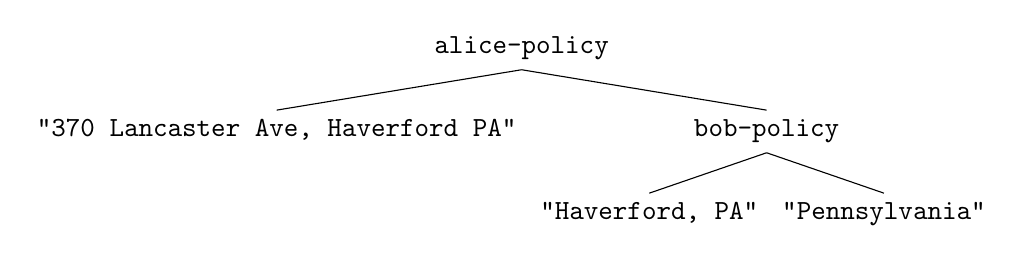
\begin{tikzpicture}
	\Tree
	[.\texttt{alice-policy}
		\texttt{"370 Lancaster Ave, Haverford PA"}
		[.\texttt{bob-policy}
			\texttt{"Haverford, PA"}
			\texttt{"Pennsylvania"}
		]
	]
	\end{tikzpicture}
	\caption{A nested facet}
	\label{figure:nested}
\end{center}
\end{figure}

Alice observes her nested facet in the usual way:

\begin{lstlisting}
(obs alice-policy "Alice" location-facet)
\end{lstlisting}

Bob must make two calls to \texttt{obs} to fully resolve the facet's value:

\begin{lstlisting}
(obs alice-policy
     "Bob"
     (obs bob-policy "Bob" location-facet))
\end{lstlisting}

As before, Bob must ensure that the policy he passes to each \texttt{obs} call matches the policy of the facet. In this case, the outer facet uses Alice's policy and the inner facet uses Bob's policy, so the calls to \texttt{obs} must be organized likewise.


\subsubsection{An example of faceted structs}
Compound data structures such as structs may be faceted. However, the behavior of faceted structs in \textsc{Racets} is somewhat counterintuitive. Take the following example:

\begin{lstlisting}
(struct employee (name position salary))
(define bob
  (employee "Bob" "manager" (fac bob-policy 70000 0)))
\end{lstlisting}

The call to the \texttt{employee} constructor is handled by \textsc{Racets} the same way that any function call is: by branching execution on both values on the facet. Consequently, the return value is \texttt{(fac bob-policy (employee "Bob" "manager" 70000) (employee "Bob" "manager" 0))}, i.e. a facet that wraps two different instantiations of the \texttt{employee} struct, rather than a structure containing a faceted value for the \texttt{salary} field, as one might expect. Bob's faceted salary can be accessed like so:

\begin{lstlisting}
(employee-salary (obs bob-policy "Bob" bob))
; or, equivalently:
(obs bob-policy "Bob" (employee-salary bob))
\end{lstlisting}

A surprising consequence is that \texttt{obs} is required to observe the name field (and any other field) of the \texttt{employee} object, even though it was not explicitly faceted in the constructor.

\begin{lstlisting}
(employee-name (obs bob-policy "Bob" bob))
\end{lstlisting}

\textsc{Racets} programs must take care to observe this subtlety when working with faceted structs.


\subsubsection{An example of faceted lists}
Using faceted values with lists involves similar complications. Consider the following example:

\begin{lstlisting}
(define grades (list))
(set! grades (cons (fac alice-policy 84 0) grades))
\end{lstlisting}

The programmer likely intended for \texttt{grades} to be of the form \texttt{(list (fac alice-policy 84 0))}, i.e. a regular list containing a single facet. However, the real value of \texttt{grades} after the \texttt{set!} operation is \texttt{(fac alice-policy (list 84) (list 0))}, because the call to \texttt{cons} is transformed into

\begin{lstlisting}
(fac alice-policy (cons 84 grades) (cons 0 grades))
\end{lstlisting}

\noindent per the standard function application transformation. Imagine another grade was added to the list, like so:

\begin{lstlisting}
(set! grades (cons (fac bob-policy 73 0) grades))
\end{lstlisting}

Then the value of the list would be

\begin{lstlisting}
(fac bob-policy
  (fac alice-policy (list 73 84) (list 73 0))
  (fac alice-policy (list 0 84) (list 0 0)))
\end{lstlisting}

\noindent encompassing four different possibilities: satisfying both Alice and Bob's policies, satisfying one or the other, or satisfying neither. The tree in figure \ref{figure:nested-list} illustrates this structure diagrammatically.

\begin{figure}[h]
\begin{center}
	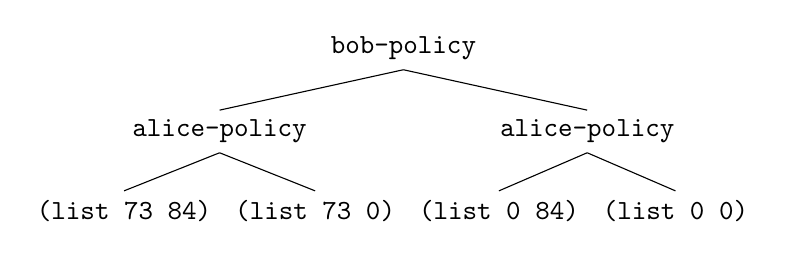
\begin{tikzpicture}
		\Tree
		[.\texttt{bob-policy}
			[.\texttt{alice-policy}
				\texttt{(list 73 84)}
				\texttt{(list 73 0)}
			]
			[.\texttt{alice-policy}
				\texttt{(list 0 84)}
				\texttt{(list 0 0)}
			]
		]
	\end{tikzpicture}
	\caption{A nested facet containing lists}
	\label{figure:nested-list}
\end{center}
\end{figure}

Programmers may find it useful to convert a faceted list into a list of non-faceted values. \texttt{obs-list} accomplishes this:

\begin{lstlisting}
(define (obs-list faceted-list policy-list arg)
  (if (empty? policy-list)
    faceted-list
    (obs
      (car policy-list)
      arg
      (obs-list
        faceted-list
        (cdr policy-list)
        arg))))])
\end{lstlisting}

\texttt{obs-list} takes in a faceted list, a list of policies which must correspond index-by-index to the policies attached to the elements of the faceted list,\footnote{Alternatively, if all elements of the list use the same policy, \texttt{obs-list} could be modified to take a single policy rather than a list.} and an argument to pass to the policy predicates. It traverses the policy tree tail-recursively, observing a single policy at each step.

This section and the previous one have illustrated usability issues with the interaction of faceted execution and data structures, stemming from the generic treatment of faceted function application. For the sake of programming ergonomics, future implementations of faceted execution may wish to not treat functional application quite so generically, so as to allow structure-creating forms like \texttt{list} and struct constructors to behave more intuitively with faceted arguments.



\section{Extending Racket with faceted execution\label{sec:lang}}
\textsc{Racets} is currently implemented as a collection of syntactic macros. In this section, I review the current implementation, and present a more flexible and powerful approach using Racket's \texttt{\#lang} mechanism, as well as a concrete proof-of-concept illustrating a crucial technique for using \texttt{\#lang} that resolves an issue with the semantics of mutable state.


\subsection{Syntactic macros}
Since syntactic macros figure heavily in the implementation of \textsc{Racets}, a brief introduction to the Racket macro system is given here. Readers are referred to the ``Fear of Macros'' tutorial \cite{fear-of-macros} for a much more comprehensive treatment.

Syntactic macros are a mechanism by which the source syntax of a program is transformed prior to execution, so that programmers may define new syntactic structures without having to modify the actual compiler or interpreter. They are a more powerful cousin of the lexical macros familiar to C and C++ programmers.

The definition of a macro resembles a function that receives a syntax object as input and returns another syntax object as output, except that \texttt{define-syntax} is used instead of \texttt{define}. The simplest possible macro returns its input unchanged:

\begin{lstlisting}
(define-syntax (identity stx) stx)
\end{lstlisting}

A macro is invoked just like a regular function:

\begin{lstlisting}
; Expands to x
(identity x)
\end{lstlisting}

At compile time, the Racket compiler searches through the source code for uses of user-defined macros, evaluates the macros where they appear, and substitutes the result into the original source code. It then continues to recursively search the syntax tree, expanding macros until no more more macros are left in the source code. This process is known as \textit{macro expansion}.

New syntax objects can be constructed with the \texttt{syntax} function or its abbreviation, \texttt{\#'}:

\begin{lstlisting}
(define-syntax (ignore-input stx)
  ; Equivalent to (syntax (displayln "ignoring input"))
  #'(displayln "ignoring input")
\end{lstlisting}

Syntax objects can be converted to and from lists. This functionality allows us to implement a macro that reverses its arguments:

\begin{lstlisting}
(define-syntax (reverse-syntax stx)
  (datum->syntax stx (reverse (cdr (syntax->datum stx)))))
\end{lstlisting}

It is necessary to pass the \texttt{cdr} of the syntax list to \texttt{reverse} (a regular Racket function that operates on lists), because the \texttt{car} of the syntax list will always be the token \texttt{reverse-syntax} itself. A programmer could use the \texttt{reverse-syntax} macro as follows:

\begin{lstlisting}
; Expands to (+ 20 22), which evaluates to 42
(reverse-syntax 20 22 +)
\end{lstlisting}

Since syntactic macros are expanded at compile-time, they are capable of things that are impossible for regular functions. \texttt{my-and}, defined below, defines the lazy boolean $and$ function, so that if \texttt{a} in \texttt{(my-and a b)} evaluates to false, then \texttt{b} is never evaluated. Lazy evaluation of this sort could not be implemented by a regular function, because a regular function has no control over the evaluation of its arguments---they are always evaluated before they are passed.

\begin{lstlisting}
(define-syntax (my-and stx)
  (syntax-case stx ()
    [(_ a b)
     #'(if a b #f)]))
\end{lstlisting}

Each identifier in the \texttt{(\_ a b)} pattern clause matches a single top-level expression (which may be an atomic value or a compound structure like a list). The underscore matches the name of the macro itself,\footnote{The use of an underscore is purely conventional, to indicate that the macro does not care about the value it captures. Racket itself treats underscores the same as any other identifier in a syntax pattern.} and the symbols \texttt{a} and \texttt{b} match arguments to the macro.

One final point about syntactic macros in Racket is that they are hygienic, meaning that identifiers introduced in the macro are protected from conflicting with identical symbols in the original source code. Consider the following macro, which increments its argument by ten:

\begin{lstlisting}
(define-syntax (add-ten stx)
  (syntax-case stx ()
    [(_ a)
     #'(let ([x 10]) (+ x a))]))
\end{lstlisting}

If \texttt{add-ten} was used in a context where an identifier \texttt{x} was already defined, e.g.

\begin{lstlisting}
(define x 32)
(add-ten x)
\end{lstlisting}

\noindent then one might expect that it would expand to

\begin{lstlisting}
; Wrong!
(define x 32)
(let ([x 10] (+ x x)))
\end{lstlisting}

\noindent so that \texttt{(add-ten x)} would counterintuitively evaluate to 20. In actual fact, the macro system rewrites the identifier \texttt{x} in the macro to a name which it can guarantee will not collide with any existing identifier in the program, as demonstrated below.

\begin{lstlisting}
; Correct -- x in the macro is rewritten as x:3
(define x 32)
(let ([x:3]) (+ x x:3))
\end{lstlisting}

At runtime the expanded macro thus correctly evaluates to 42.


\subsection{Racets with macros}
\textsc{Racets} uses macros to redefine core Racket forms to make them sensitive to faceted values. For example, the transformation of function application (for a single argument) could be implemented by

\begin{lstlisting}
(define-syntax (#%app stx)
  (syntax-parse stx
    [(_ f a)
      #'(if (facet? a)
          (fac
	    (facet-labelname a)
	    (f (facet-left a))
	    (f (facet-right a)))
	  (f a))]))
\end{lstlisting}

\noindent using the \textsc{Racets}-internal functions \texttt{facet-labelname}, \texttt{facet-left}, and \texttt{facet-right} to access the fields of the facet.

\texttt{\#\%app}, the name of the macro above, is a special form in Racket. During macro expansion, all function applications are transformed to use the \texttt{\#\%app} form, so that \texttt{(f a b)} is re-written as \texttt{(\#\%app f a b)}. This transformation occurs in plain Racket, independently of \textsc{Racets} and its macro. Defining a macro for \texttt{\#\%app} allows all function applications to be captured and transformed, which is exactly what the semantics of \textsc{Racets} require.

Other macros are provided for a subset of the core forms of Racket. See \cite{racets} for details of the implementation.


\subsubsection{Shortcomings\label{sec:shortcomings}}
Implementing \textsc{Racets} using macros suffers from two shortcomings: certain constructions involving \texttt{set!} cannot be handled correctly, and the \textsc{Racets} macros may interfere with user-defined macros.

To correctly handle \texttt{set!} forms with faceted values, the \textsc{Racets} system needs to wrap (some) identifiers with extra conditional logic. To see why, consider the following code snippet:

\begin{lstlisting}
(if k
  (set! x 100)
  (set! x 0))
\end{lstlisting}

Suppose that \texttt{k} is a facet belonging to Alice whose high-confidentiality value is true and whose low-confidentiality value is false. Upon execution of the \texttt{if} statement, the value of \texttt{x} will be a box containing \texttt{(fac alice-policy 100 0)}. However, the code is written as if \texttt{x} were an integer, so if at a later point some arithmetic operation were attempted on \texttt{x}, it would fail, because \texttt{x} is in fact a box and not an integer.

Note that the problem is not that \texttt{x} is invisibly transformed into a facet, which happens frequently in policy-agnostic faceted code and is handled by the mechanisms of faceted execution, but that it becomes a box containing a facet. To handle this case, all bare identifiers must be wrapped in logic that checks if it is a box containing a facet, and unboxes it if it is.

One might imagine that there is a \texttt{\#\%identifier} form in Racket which wraps all identifiers at some point in the macro expansion process, analogous to the \texttt{\#\%app} form for function applications. In that case, \textsc{Racet} could include a macro for \texttt{\#\%identifier} that implements the necessary logic. Unfortunately, there is no such form: identifiers are ``raw'' in the syntax and cannot be targeted individually and exclusively by a syntactic macro. A different approach must be used.

The second issue is that \textsc{Racets} may interfere with other macros, for instance if the programmer redefined the \texttt{\#\%app} form themselves. As it turns out, the same approach---the language-as-a-library approach---that solves the previous issue addresses this issue as well.


\subsection{Racets as a language-library}
All Racket files begin with a \texttt{\#lang racket} declaration. The \texttt{\#lang} statement may be used to declare other languages, e.g. \texttt{\#lang typed/racket} for Typed Racket \cite{typed-racket}, and it may be used to delegate parsing of the file to another Racket file. In the latter case, it is written as \texttt{\#lang s-exp "m.rkt"}, where \texttt{m.rkt} is the name of the Racket file to which parsing has been delegated. \texttt{m.rkt} defines syntactic macros which are used in the expansion of the file that includes the \texttt{\#lang s-exp "m.rkt"} declaration.

The languages-as-libraries approach \cite{lang-as-lib} uses \texttt{\#lang} to implement new domain-specific languages which are compatible with plain Racket code, and which are much easier to write than an entire new language, since they can reuse all the facilities exposed by the Racket compiler. The key idea of languages-as-libraries is to override the \texttt{\#\%module-begin} form , which implicitly or explicitly wraps all Racket modules, so that the entire source code of the module can be intercepted. The source code can then be passed to a Racket function called \texttt{local-expand}, which invokes the macro expansion process to expand the source code into a minimal subset of Racket called Fully-Expanded Racket \cite{fe-racket}, expanding all user-defined macros along the way.

The language-library then only needs to provide translations for the small set of core forms that constitute Fully-Expanded Racket, rather than the much larger set of forms that may appear in regular Racket, and does not need to worry about name conflicts with user-defined macros, since they have already been expanded by \texttt{local-expand}.


\subsubsection{Small example of a language-library}
The following minimal but complete example of the languages-as-libraries idea prints out the fully-expanded abstract syntax tree of a program before running it normally:

\begin{lstlisting}
#lang racket

; Fully expands the module and prints out its abstract
; syntax tree, before running it normally.
(define-syntax (module-begin stx)
  (syntax-case stx ()
    [(_ forms ...)
    (with-syntax ([(_ core-forms ...)
                   (local-expand
                     #'(#%plain-module-begin forms ...)
                     'module-begin
                     '())])
      #'(#%plain-module-begin
          (displayln '(core-forms ...))
          core-forms ...))]))

; Export everything from the regular Racket language,
; except replace #%module-begin with our own
; implementation.
(provide (except-out (all-from-out racket) #%module-begin)
          (rename-out [module-begin #%module-begin]))
\end{lstlisting}

If this program were saved in a file called \texttt{print-ast.rkt}, then other files could be written in the language by beginning with \texttt{\#lang s-exp "print-ast.rkt"}.

The file \texttt{print-ast.rkt} begins with the standard \texttt{\#lang racket} declaration, since it itself is written in Racket. It then defines a macro called \texttt{module-begin} which rewrites its argument to be

\begin{lstlisting}
#'(#%plain-module-begin
    (displayln '(core-forms ...))
    core-forms ...))]))
\end{lstlisting}

\noindent where \texttt{core-forms} is defined by the \texttt{with-syntax} clause to be the result of invoking \texttt{local-expand} on the original syntax object. The macro then outputs a \texttt{\#\%plain-module-begin} form (rather than a \texttt{\#\%module-begin}, to avoid infinite recursion) that wraps the original source syntax, after a call to \texttt{displayln} that prints at runtime the actual syntax object that was generated at compile-time.


\subsubsection{Larger example of a language-library}
As a proof-of-concept of implementing Racets with the language-as-a-library approach, this section presents a library called \texttt{wrap-ident.rkt} that rewrites identifiers in the source code in roughly the manner that the real \textsc{Racets} implementation requires.

The effect of the \texttt{wrap-ident.rkt} module is to re-write the syntax tree so that

\begin{lstlisting}
#lang s-exp "wrap-ident.rkt"

(define x 10)
(define y 32)
(displayln (+ x y))
\end{lstlisting}

\noindent becomes

\begin{lstlisting}
(define x 10)
(define y 32)
(displayln ((var-wrapper +) (var-wrapper x)
                               (var-wrapper y)))
\end{lstlisting}

\noindent where \texttt{var-wrapper} is defined with the logic outlined in section \ref{sec:shortcomings}:

\begin{lstlisting}
(define (var-wrapper v)
  (if (and (box? v) (facet? (unbox v)))
    (unbox v)
    v))
\end{lstlisting}

The core of \texttt{wrap-ident.rkt} is a procedure called \texttt{transform-syntax}, which recursively walks the program's syntax tree, detects bare identifiers, and wraps them with \texttt{var-wrapper}. Most forms in Fully-Expanded Racket can be transformed simply by recursively transforming each argument. Some forms need to be treated specially. An example is \texttt{set!}: \texttt{(set! x 10)} could not be re-written as \texttt{(set! (var-wrapper x) 10)}, as the first argument to \texttt{set!} must be a bare identifier. \texttt{transform-syntax} therefore contains patterns to match special-case forms, followed by a default case for any other list of forms, followed by a case for any individual form, which performs the actual work of identifying and re-writing identifiers. An abbreviated implementation is given here:

\begin{lstlisting}
(define (transform-syntax stx)
  (syntax-case stx ()
    ; set!
    ([head id expr]
     (check-ident #'head #'set!)
     #`(head id #,(transform-syntax #'expr)))

    ; provide
    ([head a ...]
     (check-ident #'head #'#%provide)
     stx)

    ; #%plain-lambda
    ([head formals expr ...]
     (check-ident #'head #'#%plain-lambda)
     (datum->syntax stx
                    (cons #'head
                          (cons #'formals
                                (map transform-syntax
				     (syntax-e #'(expr ...)))))))

    ; quote
    ([head datum]
     (check-ident #'head #'quote)
     #'(head datum))

    ; Any other list of forms.
    ([a b ...]
     (datum->syntax stx (cons #'a (map transform-syntax
                                           (syntax-e #'(b ...))))))

    ; Any other individual form.
    (default
      (if (identifier? #'default)
        #`(var-wrapper #,#'default)
        #'default))))
\end{lstlisting}

The code listing above is not exhaustive: special cases for \texttt{let-values} and \texttt{letrec-values}, among others, are omitted for the sake of brevity as their syntax requires complex pattern matching.

Each pattern has a guard clause that uses the helper function \texttt{check-ident} to check that the head of the matched form is bound to the same variable as the form to be re-written. \texttt{check-ident} is defined below. It uses \texttt{free-identifier=?} to check its argument's binding. It is important to use this function rather than comparing the textual content of the identifiers, because Racket does not guarantee the textual content will be the same. An identifier may have the surface form of \texttt{lambda} but actually be bound to \texttt{\#\%plain-lambda}. \texttt{free-identifier=?}, unlike a comparison of symbolic equality, is sensitive to this distinction.

\begin{lstlisting}
(define (check-ident ident expected)
  (and (identifier? ident)
        (free-identifier=? ident expected)))
\end{lstlisting}

The final piece is the whole-module rewrite rule:

\begin{lstlisting}
(define-syntax (module-begin stx)
  ; Intercept the entire module and transform it using
  ; `transform-syntax` on the fully-expanded syntax tree
  ; (which ensures that user macros are expanded first).
  (syntax-case stx ()
    [(_ forms ...)
     (let ([expanded
            (local-expand #'(#%plain-module-begin forms ...)
	                  'module-begin
			  '())])
       (transform-syntax expanded))]))

(provide (except-out (all-from-out racket) #%module-begin)
          (rename-out [module-begin #%module-begin]))
\end{lstlisting}

The \texttt{module-begin} macro invokes \texttt{local-expand} on the module contents, and then calls \texttt{transform-syntax} to transform the resulting fully-expanded syntax tree.

If this proof-of-concept were extended to handle the remaining core forms of Fully-Expanded Racket, and augmented with the original set of \textsc{Racets} macros, it would yield a more robust implementation of faceted execution in Racket.



\section{Type theory\label{sec:types}}
Since \textsc{Racets}, like Racket, is dynamically typed, errors in the use of faceted values (such as supplying the wrong policy to \texttt{obs}) are not caught until the invalid operation is attempted at runtime. A static type system for faceted values could detect many programmer errors at compile time. This section presents an introduction to formal type theory and indicates how it might be applied to faceted execution.

A type system is ``a tractable syntactic method for proving the absence of certain program behaviors by classifying phrases according to the kinds of values they compute'' \cite{types}. The program behaviors that a type system are meant to prevent are generally what are called type errors: attempted operations on values for which the operation is not defined.

Naturally, type systems cannot catch all errors: some undesirable program behaviors cannot be detected (e.g., looping infinitely is not detectable due to the uncomputability of the halting problem), and type systems will sometimes reject constructs which are actually safe. Nonetheless, a well-designed type system is an effective tool for catching programmer errors.

Formal type theory will be presented through the example of the typed lambda calculus. The following exposition is based on chapter 9 of \cite{types}.

The lambda calculus is a simple mathematical model of computation in which the only data type is the function and the only operation is function application. Despite its simplicity, any possible computation can be expressed in the lambda calculus, per the Church-Turing thesis. The syntax of the lambda calculus comprises three kinds of terms: variables ($x$, $y$, etc.), anonymous functions, also known as abstractions ($\lambda x . x$), and function applications ($t\ t$). The notation $\lambda x . x$ is equivalent to the more traditional notation of $f(x) = x$, with the advantage of not requiring the function to be named. Function application of the form $t_1\ t_2$ is equivalent notationally to $t_1(t_2)$, i.e. the application of the function $t_1$ to the argument $t_2$. The body of a lambda function may contain any of the three syntactic forms of the language, so for example $\lambda x . \lambda y . (\lambda z . z\ x)$ is a valid term in the lambda calculus whose outermost abstraction contains another abstraction, which in turn contains an application ($\lambda z . z$) to a variable ($x$). For clarity, the application is wrapped in parentheses.

The typed lambda calculus has the same syntax as the untyped lambda calculus, except that lambda abstractions carry a type annotation for their parameter, written as $\lambda x: T . x$, where $T$ is a type. A \textit{type annotation} is an annotation supplied by the programmer that indicates the intended type of a variable or expression. Not all typed languages require type annotations, but requiring them simplifies the specification of the type system.

A type system for the lambda calculus (and indeed for any programming language) must assign a type to each syntactic construction in the language. These assignments are formally known as type rules. Type rules are written in the form

\[
\frac{\text{hypotheses}}
{\text{conclusion}}
\]

\noindent where \textit{hypotheses} is a set of assumptions and \textit{conclusion} is a type judgment that follows from the hypotheses.

The rule for the types of variables in the lambda calculus is\footnote{The type rules are taken from Figure 9-1 on p. 103 of \cite{types}.}

\[
\frac{x : T \in \Gamma}
{\Gamma \vdash x : T}
\]

$\Gamma$ stands for an assignment function that maps from a finite number of variable names to their values. The notation $\Gamma \vdash t : T$ expresses the three-place relation that syntactic term $t$ has type $T$ given the assignment $\Gamma$. The type rule for variables simply states that if a variable is paired with a certain type $T$ in the assignment function, then $T$ is the variable's type.

The rule for lambda abstraction is a bit more complicated:

\[
\frac{\Gamma, x : T_1 \vdash t_2 : T_2}
{\Gamma \vdash \lambda x : T_1 . t_2 : T_1 \to T_2}
\]

In the hypothesis, the expression $\Gamma, x : T_1$ should be read as ``$\Gamma$ augmented with the assignment of type $T_1$ to $x$.'' It is assumed that the variable $x$ is not already in $\Gamma$; if it is, it can be renamed. The full hypothesis of the abstraction rule states that the body of the lambda function has type $T_2$ with the given assignment function. The conclusion of the abstraction rule states that the lambda function as a whole has the complex type $T_1 \to T_2$, a function from values of type $T_1$ to values of type $T_2$.

Finally, the last syntactic form of the language, application, has the type rule

\[
\frac{\Gamma \vdash t_1 : T_{11} \to T_{12}\ \ \ \ \ \ \Gamma \vdash t_2 : T_{11}}
{\Gamma \vdash t_1\ t_2 : T_{12}}
\]

Given that the function has type $T_{11} \to T_{12}$ in $\Gamma$, and the argument has type $T_{11}$, then the expression as a whole has type $T_{12}$.

The three type rules presented above can be applied to any expression in the typed lambda calculus to detect whether it is well-typed, and if it is, to determine its concrete type. Thus the type system is able to statically detect type errors in the lambda calculus.

Type systems for real programming languages are significantly more complex, but involve the same basic formalism of inference rules and type judgments for each syntactic form in the language. As such, this formalism could be deployed to augment \textsc{Racets} with a static type system that detects programming errors specific to faceted execution.



\section{Abstract interpretation\label{sec:ai}}
Another practical problem with faceted execution is that faceted code can run significantly more more slowly than non-faceted code. Functions applied to facets must be evaluated twice, once with the high-confidentiality value and once with the low-confidentiality value, resulting in a performance hit for faceted code.\footnote{It also complicates the use of functions with side-effects, which is an open problem in \textsc{Racets}.} This performance hit can be mitigated by static analysis. A static analyzer might, for instance, be able to prove that a facet is only ever resolved to its high-confidentiality value, in which case that value could be substituted for the facet as a whole, skipping double evaluation wherever it is passed to a function.

One technique for static analysis is abstract interpretation \cite{abstract-inter}, wherein the computation of a program is modeled with abstract objects (e.g., the abstract category ``negative number'' instead of the concrete value $-10$) so that semantic properties of the program can be reasoned about \cite{ai-original}.



\subsection{Deriving abstract interpreters from abstract machines}
Abstract interpreters can be mechanically derived from abstract machines using a technique presented in \cite{aam}. An \textit{abstract machine} is a formal mathematical object that models a computing machine. A Turing machine is perhaps the most familiar example of an abstract machine.

Three abstract machines of increasing resemblance to real-world technology will be presented here: the CEK, CESK, and CESK* machines. Though the language that these machines evaluate (the untyped lambda calculus) is superficially very different from real programming languages, in principle the mechanisms of function definition, application, and lexical closure are the core of most actual languages, and at any rate the lambda calculus is much closer to a modern programming language than the finite transition systems that underlie the computation of a Turing machine are.

The CEK machine has three elements in its state: $c$, an expression in the lambda calculus; $\rho$, an environment that maps from symbols to values; and $\kappa$, a continuation (the acronym ``CEK'' stands for the elements of the state). All values in the lambda calculus are closures, which are pairs of functions and environments.

Continuations are mathematical structures for representing control flow. Intuitively, a continuation encapsulates what the machine should do next after evaluating the current expression. For the lambda calculus, the sequence of machine operations is very simple, as only function application (of the three syntactic terms) requires any control flow at all: the function is evaluated first, followed by the argument, and then the body of the function. At each step, the continuation stores what the next step is.

In the CEK machine, continuations come in three forms: $\textbf{ar}(e, \rho, \kappa)$, $\textbf{fn}((\lambda x.e), \rho, \kappa)$, and $\textbf{mt}$. The first form represents evaluating an argument $e$, and the second form represents evaluating the body of a function. The third form is the empty continuation, which halts execution. In the first two forms, $\rho$ is the environment in which the expression is to be evaluated, and $\kappa$ is the continuation that is to be followed afterwards.

The entirety of the operation of the CEK machine is described by four rules that map from one machine state (a 3-tuple of expression, environment and continuation) to another.\footnote{These rules are reproduced and slightly modified from Figure 1 on p. 2 of \cite{aam}. See \cite{cek} for a different formulation of the CEK machine's transition rules.} The first rule is for evaluating variables:

% Evaluating a symbol (CEK)
$$
\text{1. }
\langle x, \rho, \kappa \rangle
\to
\langle v, \rho', \kappa \rangle,
\text{ given that $x$ is bound to $(v, \rho')$ in $\rho$}
$$

The new expression to evaluate is the closure that the variable maps to in the environment. The old environment is replaced with the closure's environment. The original continuation is preserved, since evaluating variables does not involve a change in control flow.

The second rule is for evaluating function applications:

% Evaluating an application (CEK)
$$
\text{2. }
\langle (e_0\ e_1), \rho, \kappa \rangle
\to
\langle e_0, \rho, \textbf{ar}(e_1, \rho, \kappa) \rangle
$$

The first expression to be evaluated in a function application is the function itself, so this function ($e_0$ in the formula) becomes the expression in the output state. The environment in which the function is evaluated is the same in which the function application as a whole is evaluated, so $\rho$ is preserved. The new continuation directs the abstract machine to evaluate the argument next, in the same environment, followed by the original continuation $\kappa$.

The last two rules handle the evaluation of values, i.e. closures. If the current continuation is of the \textbf{ar} form, the following rule applies:

% Evaluating an argument (CEK)
$$
\text{3. }
\langle v, \rho, \textbf{ar}(e, \rho', \kappa) \rangle
\to
\langle e, \rho', \textbf{fn}(v, \rho, \kappa) \rangle
$$

The old expression and environment are replaced with the expression and environment provided by the continuation. After evaluating the argument, we want to evaluate the body of the function, so we provide a \textbf{fn} continuation that encapsulates the function itself, the original environment, and the original continuation.

The last rule applies to evaluating values with an \textbf{fn} continuation:

% Evaluating a function (CEK)
$$
\text{4. }
\langle v, \rho, \textbf{fn}((\lambda x.e), \rho', \kappa) \rangle
\to
\langle e, \rho'[x \mapsto (v, \rho)], \kappa \rangle
$$

The body of the function, $e$, is the next expression to be evaluated, so it goes in the expression slot of the output state. The environment is the one indicated by the old continuation, augmented with a binding of the function's parameter to the value of its argument, which must be in the old expression slot per the previous rule. We preserve the old continuation.

In addition to state-mapping rules, an abstract machine needs an \textit{injection function} that provides its initial state, given an expression to evaluate. For the CEK machine, the injection function is defined as

$$ inj_{CEK}(e) = \langle e, \emptyset, \textbf{mt} \rangle $$

The environment is initially empty, and the continuation is \textbf{mt}, because the next thing to do after evaluating the expression is to halt.

The transition rules may be clarified by walking through their application in a concrete example. Suppose we want to evaluate the lambda expression $(\lambda x.x\ \lambda y.y)$ (which should evaluate to $\lambda y.y$). We begin by applying $inj_{CEK}$ to get the initial state of the machine:

$$ s_0 = \langle (\lambda x.x\ \lambda y.y), \emptyset, \textbf{mt} \rangle $$

$s_0$ matches rule 2, so we apply the rule to yield the next state. As expected, we are evaluating the function ($\lambda x.x$) first, and the continuation indicates that we must evaluate the argument afterwards:

$$ s_1 = \langle \lambda x.x, \emptyset, \textbf{ar}(\lambda y.y, \emptyset, \textbf{mt}) \rangle $$

$s_1$ in turn matches rule 3, which we apply below. We are now evaluating the argument, and the continuation tells us that evaluating the body of the function is next.

$$ s_2 = \langle \lambda y.y, \emptyset, \textbf{fn}(\lambda x.x, \emptyset, \textbf{mt}) \rangle $$

$s_2$ matches rule 4. We bind the value of the argument to the function's parameter in the environment, and evaluate the body in this new environment. Since evaluating the body is the last step in evaluating the function application as a whole, the continuation points to the next thing (halt computation) as expected.

$$ s_3 = \langle x, \{ x: (\lambda y.y, \emptyset) \}, \textbf{mt} \rangle $$

$s_3$ matches rule 1:

$$ s_4 = \langle \lambda y.y, \emptyset, \textbf{mt} \rangle $$

We have now reached a value with a continuation of \textbf{mt}, so computation halts. As expected, the value $\lambda y.y$ is in the expression slot of the final slot.

The CEK machine can be augmented with a store to represent mutable state. A store maps addresses to values, and can be imagined as the abstract mathematical equivalent of a computer's memory unit.

The CEK machine augmented with a store is known as the CESK machine \cite{cesk}. \cite{aam} present a slight modification to the CESK machine, in which continuations are allocated in the store in order to make the machine more amenable to conversion into an abstract interpreter. This machine is known as the CESK* machine.

The state of the CESK* machine consists of $c, \rho, \sigma, a$, where $c$ is defined as for the CEK machine, $\rho$ is modified to map from symbols to addresses instead of values, the store $\sigma$ maps from addresses to values, and $a$ is the address of a continuation in the store.\footnote{For the regular CESK machine, $a$ is instead $\kappa$ with the same meaning as for the CEK machine.}

The injection function for the CESK machine is slightly (but only slightly) more complex than $inj_{CESK}$:

$$ inj_{CESK*}(e) = \langle e, \emptyset, \{ a_0: \textbf{mt} \}, a_0 \rangle $$

The environment is initially empty. The store contains the \textbf{mt} continuation, and the continuation address slot points at this continuation.

The four rules for the behavior of the CESK* machine are likewise similar.\footnote{These rules are reproduced and slightly modified from Figure 3 on p. 4 of \cite{aam}.} Several of the rules use $alloc()$, a function which returns a new address in the store that has not been used yet.

The first rule, for evaluating variables, is almost identical:

% Evaluating a symbol (CESK*)
$$
\text{1. }
\langle x, \rho, \sigma, a \rangle
\to
\langle v, \rho', \sigma, a \rangle,
\text{ given that $x$ is bound to $(v, \rho')$ in $\rho$}
$$

The second rule, for function application, differs only in that the continuation is allocated in the store:

% Evaluating an application (CESK*)
$$
\text{2. }
\langle (e_0\ e_1), \rho, \sigma, a \rangle
\to
\langle e_0, \rho, \sigma[b \mapsto \textbf{ar}(e_1, \rho, a)], b \rangle
\text{ where $b = alloc()$}
$$

The third and fourth rules again differ only in the use of the store:

% Evaluating an argument (CESK*)
$$
\text{3. }
\langle v, \rho, \sigma, a \rangle
\to
\langle e, \rho', \sigma[b \mapsto \textbf{fn}(v, \rho, c)], b \rangle
\text{ where $b = alloc()$}
$$
$$
\text{given that $a$ maps to $\textbf{ar}(e, \rho', c)$ in $\sigma$}
$$

% Evaluating a function (CESK*)
$$
\text{4. }
\langle v, \rho, \sigma, a \rangle
\to
\langle e, \rho'[x \mapsto b], \sigma[b \mapsto (v, \rho)], c \rangle
$$
$$
\text{given that $a$ maps to $\textbf{fn}((\lambda x.e), \rho', c)$ in $\sigma$}
$$

The CESK* machine is thus quite similar in principle to the CEK machine, but the use of a store for values and continuations allow the construction of an abstract interpretation from the CESK* machine to proceed more smoothly.\footnote{In \cite{aam}, the authors tweak the CESK* machine to use time-stamps before they derive the abstract interpreter. For simplicity of exposition, this modification has been omitted.} The reason is that abstract interpretation must terminate to be useful in practice. The abstract interpreter can enforce that the store is finite, so moving values and continuations to the store ensures that the interpretation will terminate, which otherwise could not be guaranteed if environments and continuations were arbitrary recursive structures unbound to any finite container.

The abstract CESK* interpreter is defined similarly to the CESK* machine, except that the store maps to sets of values instead of concrete values, and it transitions between sets of machine states instead of single states. The interpreter continues transitioning until it reaches a fixed-point, when applying its transition function to each individual states yields the original set. Once the abstract CESK* interpreter has terminated, its store can be inspected to determine semantic properties of the program.

Formally, the abstract CESK* interpreter is a 4-tuple $(c, \rho, \hat{\sigma}, a)$, where $c$, $\rho$ and $a$ are defined the same as for the CESK* machine, and $\hat{\sigma}$ maps from addresses to sets of values instead of single values.

The behavior of the abstract CESK* interpreter is defined by four transition rules. Some of these rules make use of an allocation function $\widehat{alloc} : \hat{\Sigma} \times Kont \to Addr$, which takes in an abstract interpreter state and a continuation in order to decide what address to return. Its implementation is left unspecified here.

The first transition rule, for variables, is essentially identical to the analogous rule for the CESK* machine:\footnote{These rules are reproduced from Figure 5 on p. 5 of \cite{aam} and modified to apply to the CESK* interpreter instead of the time-stamped CESK* interpreter originally presented in the paper.}

% Evaluating a symbol (abstract CESK*)
$$
\text{1. }
\langle x, \rho, \hat{\sigma}, a \rangle
\to
\langle v, \rho', \hat{\sigma}, a \rangle,
\text{ given that $(v, \rho') \in \rho(x)$}
$$

The remaining three rules are where the important difference between the CESK* machine and the abstract CESK* interpreter come to light. Rather than assigning directly to the store, the new mapping is unioned with the existing store, so that it contains both the new mapping and any old mapping that the new mapping might have otherwise overwritten.

% Evaluating an application (abstract CESK*)
$$
\text{2. }
\langle (e_0\ e_1), \rho, \hat{\sigma}, a \rangle
\to
\langle e_0, \rho, \hat{\sigma} \cup [b \mapsto \textbf{ar}(e_1, \rho, a)], b \rangle
\text{ where $b = \widehat{alloc}(\varsigma, \kappa)$}
$$
% Evaluating an argument (abstract CESK*)
$$
\text{3. }
\langle v, \rho, \hat{\sigma}, a \rangle
\to
\langle e, \rho', \hat{\sigma} \cup [b \mapsto \textbf{fn}(v, \rho, c)], b \rangle
\text{ where $b = \widehat{alloc}(\varsigma, \kappa)$}
$$
$$
\text{given that } \textbf{ar}(e, \rho', c) \in \hat{\sigma}(a)
$$
% Evaluating a function (CESK*)
$$
\text{4. }
\langle v, \rho, \hat{\sigma}, a \rangle
\to
\langle e, \rho'[x \mapsto b], \hat{\sigma} \cup [b \mapsto (v, \rho)], c \rangle
$$
$$
\text{given that } \textbf{fn}((\lambda x.e), \rho', c) \in \hat{\sigma}(a)
$$

Other than modifying the store in the manner described above, the transition rules for the abstract CESK* interpreter are more or less the same as for the CESK* machine.

When the abstract interpreter has terminated, its store can be inspected to reason about the semantics of the program. For example, if every element of the set that address $a$ maps to is a negative number, then we can conclude that the variable or variables corresponding to $a$ will always be negative.

% TODO: Awkward
We are now in a position to understand why store-allocated continuations are crucial for converting the CESK* machine into an abstract interpreter. Abstract interpretation must terminate to be useful in practice. One way of enforcing termination is by keeping the store finite, which can be accomplished by defining the allocation function $\widehat{alloc}$ in such a way that its co-domain is finite. If continuations were outside of the store, they would be recursive structures that could potentially nest infinitely. Once moved to the store, their finite-ness is guaranteed by the broader finite-ness of the store itself.


\subsection{Abstract interpretation of Racets}
Recall that the original motivation for abstract interpretation was to improve the runtime performance of programs by statically proving facts about the program's semantics that could be used for compile-time optimizations. The extended \textsc{Racets} implementation presented in section \ref{sec:lang} has a particularly high runtime overhead, because every variable reference must be wrapped in a conditional. A simple module like

\begin{lstlisting}
#lang s-exp "racets.rkt"

(define x 10)
(define y 32)
(displayln (+ x y))
\end{lstlisting}

\noindent would balloon into

\begin{lstlisting}
#lang s-exp "racets.rkt"

(define x 10)
(define y 32)
(
 ; displayln
 (if (and (box? displayln) (facet? (unbox displayln)))
      (unbox displayln)
      displayln)
  ; x
  (if (and (box? x) (facet? (unbox x)))
    (unbox x)
    x)

  ; y
  (if (and (box? y) (facet? (unbox y)))
    (unbox y)
    y))
\end{lstlisting}

Of course, none of these conditionals are actually necessary, because neither \texttt{displayln}, nor \texttt{x}, nor \texttt{y} will ever be boxed facets at runtime.

An abstract interpreter for \textsc{Racets} would have (at a minimum) abstract domains for box and unboxed values, and for faceted and non-faceted values. If the abstract interpreter were able to determine that a particular value was never boxed, or never faceted, then the extra apparatus of faceted execution (like the conditional checks in the code snippet above) could be eliminated at compile time.

The level of precision that the abstract interpreter attains with its analysis can have a substantial effect on performance. For example, if a certain function is sometimes applied to faceted values and sometimes applied to regular values, the abstract interpreter may or may not be able to identify the call sites that require special handling of the faceted execution, and those that can be run normally. In general, the more fine-grained the conclusions the abstract interpreter can draw, the greater the improvement of performance time, at the cost of slower analysis and a more complex abstract interpreter.

Actually deriving an abstract interpreter for \textsc{Racets} (bridging the high-level description in this section with the low-level details in the previous section) is beyond the scope of this undergraduate thesis. See \cite{abstract-inter} for current work in this area.



\section{Conclusion\label{sec:conclusion}}
The primary novel contribution of this thesis is the application of the language-as-a-library technique to \textsc{Racets} in order to correctly handle mutable state and improve interoperability with non-faceted code. Two other issues in the ergonomics of faceted execution have been discussed at some length: type safety, and runtime efficiency. I have shown that static typing and abstract interpretation could mitigate these issues.

Further research may proceed in a number of directions. The presentation of static typing and abstract interpretation here has been extremely preliminary, and the details of their concrete implementation in \textsc{Racets} or in other faceted-execution systems remains to be fleshed out. The proof-of-concept of re-writing \textsc{Racets} as a \texttt{\#lang}-style language will need to be extended with the existing \textsc{Racets} macros that implement the primitives of faceted execution.

The theory and techniques reviewed in this thesis should contribute to the ergonomics of writing code with faceted execution, and thus in turn to safeguarding the privacy of software users.



\section*{Acknowledgements}
I would like to thank my thesis advisor, Kristopher Micinski, and my second faculty reader, Steven Lindell, for their valuable feedback and guidance on this project.



\bibliography{thesis}

\end{document}
